% Graphic for TeX using PGF
% Title: /home/budnyjj/univer/GIT/diploma/b/design/diagrams/bl_general.dia
% Creator: Dia v0.97.3
% CreationDate: Sun May  8 01:50:49 2016
% For: budnyjj
% \usepackage{tikz}
% The following commands are not supported in PSTricks at present
% We define them conditionally, so when they are implemented,
% this pgf file will use them.
\ifx\du\undefined
  \newlength{\du}
\fi
\setlength{\du}{15\unitlength}
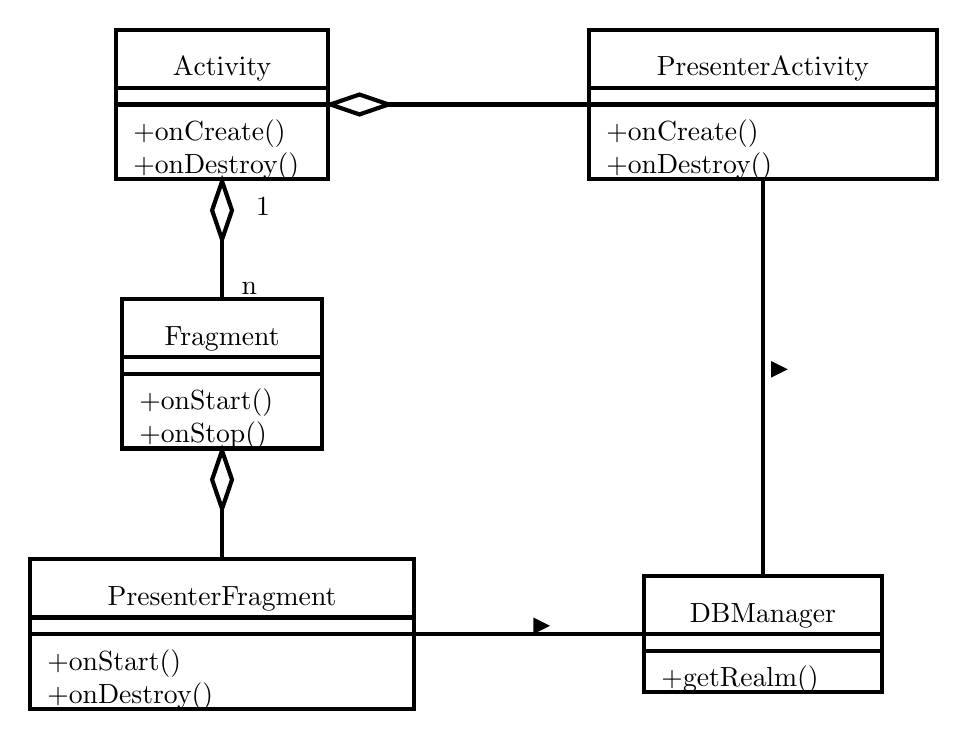
\begin{tikzpicture}
\pgftransformxscale{1.000000}
\pgftransformyscale{-1.000000}
\definecolor{dialinecolor}{rgb}{0.000000, 0.000000, 0.000000}
\pgfsetstrokecolor{dialinecolor}
\definecolor{dialinecolor}{rgb}{1.000000, 1.000000, 1.000000}
\pgfsetfillcolor{dialinecolor}
\pgfsetlinewidth{0.100000\du}
\pgfsetdash{}{0pt}
\definecolor{dialinecolor}{rgb}{1.000000, 1.000000, 1.000000}
\pgfsetfillcolor{dialinecolor}
\fill (7.321506\du,3.788837\du)--(7.321506\du,5.188837\du)--(12.441506\du,5.188837\du)--(12.441506\du,3.788837\du)--cycle;
\definecolor{dialinecolor}{rgb}{0.000000, 0.000000, 0.000000}
\pgfsetstrokecolor{dialinecolor}
\draw (7.321506\du,3.788837\du)--(7.321506\du,5.188837\du)--(12.441506\du,5.188837\du)--(12.441506\du,3.788837\du)--cycle;
% setfont left to latex
\definecolor{dialinecolor}{rgb}{0.000000, 0.000000, 0.000000}
\pgfsetstrokecolor{dialinecolor}
\node at (9.881506\du,4.738837\du){Activity};
\definecolor{dialinecolor}{rgb}{1.000000, 1.000000, 1.000000}
\pgfsetfillcolor{dialinecolor}
\fill (7.321506\du,5.188837\du)--(7.321506\du,5.588837\du)--(12.441506\du,5.588837\du)--(12.441506\du,5.188837\du)--cycle;
\definecolor{dialinecolor}{rgb}{0.000000, 0.000000, 0.000000}
\pgfsetstrokecolor{dialinecolor}
\draw (7.321506\du,5.188837\du)--(7.321506\du,5.588837\du)--(12.441506\du,5.588837\du)--(12.441506\du,5.188837\du)--cycle;
\definecolor{dialinecolor}{rgb}{1.000000, 1.000000, 1.000000}
\pgfsetfillcolor{dialinecolor}
\fill (7.321506\du,5.588837\du)--(7.321506\du,7.388837\du)--(12.441506\du,7.388837\du)--(12.441506\du,5.588837\du)--cycle;
\definecolor{dialinecolor}{rgb}{0.000000, 0.000000, 0.000000}
\pgfsetstrokecolor{dialinecolor}
\draw (7.321506\du,5.588837\du)--(7.321506\du,7.388837\du)--(12.441506\du,7.388837\du)--(12.441506\du,5.588837\du)--cycle;
% setfont left to latex
\definecolor{dialinecolor}{rgb}{0.000000, 0.000000, 0.000000}
\pgfsetstrokecolor{dialinecolor}
\node[anchor=west] at (7.471506\du,6.288837\du){+onCreate()};
% setfont left to latex
\definecolor{dialinecolor}{rgb}{0.000000, 0.000000, 0.000000}
\pgfsetstrokecolor{dialinecolor}
\node[anchor=west] at (7.471506\du,7.088837\du){+onDestroy()};
\pgfsetlinewidth{0.100000\du}
\pgfsetdash{}{0pt}
\definecolor{dialinecolor}{rgb}{1.000000, 1.000000, 1.000000}
\pgfsetfillcolor{dialinecolor}
\fill (18.716758\du,3.788837\du)--(18.716758\du,5.188837\du)--(27.104258\du,5.188837\du)--(27.104258\du,3.788837\du)--cycle;
\definecolor{dialinecolor}{rgb}{0.000000, 0.000000, 0.000000}
\pgfsetstrokecolor{dialinecolor}
\draw (18.716758\du,3.788837\du)--(18.716758\du,5.188837\du)--(27.104258\du,5.188837\du)--(27.104258\du,3.788837\du)--cycle;
% setfont left to latex
\definecolor{dialinecolor}{rgb}{0.000000, 0.000000, 0.000000}
\pgfsetstrokecolor{dialinecolor}
\node at (22.910508\du,4.738837\du){PresenterActivity};
\definecolor{dialinecolor}{rgb}{1.000000, 1.000000, 1.000000}
\pgfsetfillcolor{dialinecolor}
\fill (18.716758\du,5.188837\du)--(18.716758\du,5.588837\du)--(27.104258\du,5.588837\du)--(27.104258\du,5.188837\du)--cycle;
\definecolor{dialinecolor}{rgb}{0.000000, 0.000000, 0.000000}
\pgfsetstrokecolor{dialinecolor}
\draw (18.716758\du,5.188837\du)--(18.716758\du,5.588837\du)--(27.104258\du,5.588837\du)--(27.104258\du,5.188837\du)--cycle;
\definecolor{dialinecolor}{rgb}{1.000000, 1.000000, 1.000000}
\pgfsetfillcolor{dialinecolor}
\fill (18.716758\du,5.588837\du)--(18.716758\du,7.388837\du)--(27.104258\du,7.388837\du)--(27.104258\du,5.588837\du)--cycle;
\definecolor{dialinecolor}{rgb}{0.000000, 0.000000, 0.000000}
\pgfsetstrokecolor{dialinecolor}
\draw (18.716758\du,5.588837\du)--(18.716758\du,7.388837\du)--(27.104258\du,7.388837\du)--(27.104258\du,5.588837\du)--cycle;
% setfont left to latex
\definecolor{dialinecolor}{rgb}{0.000000, 0.000000, 0.000000}
\pgfsetstrokecolor{dialinecolor}
\node[anchor=west] at (18.866758\du,6.288837\du){+onCreate()};
% setfont left to latex
\definecolor{dialinecolor}{rgb}{0.000000, 0.000000, 0.000000}
\pgfsetstrokecolor{dialinecolor}
\node[anchor=west] at (18.866758\du,7.088837\du){+onDestroy()};
\pgfsetlinewidth{0.100000\du}
\pgfsetdash{}{0pt}
\definecolor{dialinecolor}{rgb}{1.000000, 1.000000, 1.000000}
\pgfsetfillcolor{dialinecolor}
\fill (7.465256\du,10.277349\du)--(7.465256\du,11.677349\du)--(12.297756\du,11.677349\du)--(12.297756\du,10.277349\du)--cycle;
\definecolor{dialinecolor}{rgb}{0.000000, 0.000000, 0.000000}
\pgfsetstrokecolor{dialinecolor}
\draw (7.465256\du,10.277349\du)--(7.465256\du,11.677349\du)--(12.297756\du,11.677349\du)--(12.297756\du,10.277349\du)--cycle;
% setfont left to latex
\definecolor{dialinecolor}{rgb}{0.000000, 0.000000, 0.000000}
\pgfsetstrokecolor{dialinecolor}
\node at (9.881506\du,11.227349\du){Fragment};
\definecolor{dialinecolor}{rgb}{1.000000, 1.000000, 1.000000}
\pgfsetfillcolor{dialinecolor}
\fill (7.465256\du,11.677349\du)--(7.465256\du,12.077349\du)--(12.297756\du,12.077349\du)--(12.297756\du,11.677349\du)--cycle;
\definecolor{dialinecolor}{rgb}{0.000000, 0.000000, 0.000000}
\pgfsetstrokecolor{dialinecolor}
\draw (7.465256\du,11.677349\du)--(7.465256\du,12.077349\du)--(12.297756\du,12.077349\du)--(12.297756\du,11.677349\du)--cycle;
\definecolor{dialinecolor}{rgb}{1.000000, 1.000000, 1.000000}
\pgfsetfillcolor{dialinecolor}
\fill (7.465256\du,12.077349\du)--(7.465256\du,13.877349\du)--(12.297756\du,13.877349\du)--(12.297756\du,12.077349\du)--cycle;
\definecolor{dialinecolor}{rgb}{0.000000, 0.000000, 0.000000}
\pgfsetstrokecolor{dialinecolor}
\draw (7.465256\du,12.077349\du)--(7.465256\du,13.877349\du)--(12.297756\du,13.877349\du)--(12.297756\du,12.077349\du)--cycle;
% setfont left to latex
\definecolor{dialinecolor}{rgb}{0.000000, 0.000000, 0.000000}
\pgfsetstrokecolor{dialinecolor}
\node[anchor=west] at (7.615256\du,12.777349\du){+onStart()};
% setfont left to latex
\definecolor{dialinecolor}{rgb}{0.000000, 0.000000, 0.000000}
\pgfsetstrokecolor{dialinecolor}
\node[anchor=west] at (7.615256\du,13.577349\du){+onStop()};
\pgfsetlinewidth{0.100000\du}
\pgfsetdash{}{0pt}
\definecolor{dialinecolor}{rgb}{1.000000, 1.000000, 1.000000}
\pgfsetfillcolor{dialinecolor}
\fill (5.249006\du,16.547760\du)--(5.249006\du,17.947760\du)--(14.514006\du,17.947760\du)--(14.514006\du,16.547760\du)--cycle;
\definecolor{dialinecolor}{rgb}{0.000000, 0.000000, 0.000000}
\pgfsetstrokecolor{dialinecolor}
\draw (5.249006\du,16.547760\du)--(5.249006\du,17.947760\du)--(14.514006\du,17.947760\du)--(14.514006\du,16.547760\du)--cycle;
% setfont left to latex
\definecolor{dialinecolor}{rgb}{0.000000, 0.000000, 0.000000}
\pgfsetstrokecolor{dialinecolor}
\node at (9.881506\du,17.497760\du){PresenterFragment};
\definecolor{dialinecolor}{rgb}{1.000000, 1.000000, 1.000000}
\pgfsetfillcolor{dialinecolor}
\fill (5.249006\du,17.947760\du)--(5.249006\du,18.347760\du)--(14.514006\du,18.347760\du)--(14.514006\du,17.947760\du)--cycle;
\definecolor{dialinecolor}{rgb}{0.000000, 0.000000, 0.000000}
\pgfsetstrokecolor{dialinecolor}
\draw (5.249006\du,17.947760\du)--(5.249006\du,18.347760\du)--(14.514006\du,18.347760\du)--(14.514006\du,17.947760\du)--cycle;
\definecolor{dialinecolor}{rgb}{1.000000, 1.000000, 1.000000}
\pgfsetfillcolor{dialinecolor}
\fill (5.249006\du,18.347760\du)--(5.249006\du,20.147760\du)--(14.514006\du,20.147760\du)--(14.514006\du,18.347760\du)--cycle;
\definecolor{dialinecolor}{rgb}{0.000000, 0.000000, 0.000000}
\pgfsetstrokecolor{dialinecolor}
\draw (5.249006\du,18.347760\du)--(5.249006\du,20.147760\du)--(14.514006\du,20.147760\du)--(14.514006\du,18.347760\du)--cycle;
% setfont left to latex
\definecolor{dialinecolor}{rgb}{0.000000, 0.000000, 0.000000}
\pgfsetstrokecolor{dialinecolor}
\node[anchor=west] at (5.399006\du,19.047760\du){+onStart()};
% setfont left to latex
\definecolor{dialinecolor}{rgb}{0.000000, 0.000000, 0.000000}
\pgfsetstrokecolor{dialinecolor}
\node[anchor=west] at (5.399006\du,19.847760\du){+onDestroy()};
\pgfsetlinewidth{0.100000\du}
\pgfsetdash{}{0pt}
\pgfsetmiterjoin
\pgfsetbuttcap
{
\definecolor{dialinecolor}{rgb}{0.000000, 0.000000, 0.000000}
\pgfsetfillcolor{dialinecolor}
% was here!!!
\definecolor{dialinecolor}{rgb}{0.000000, 0.000000, 0.000000}
\pgfsetstrokecolor{dialinecolor}
\draw (12.491825\du,5.588837\du)--(13.241825\du,5.588837\du)--(18.616499\du,5.588837\du)--(18.666499\du,5.588837\du);
}
\definecolor{dialinecolor}{rgb}{0.000000, 0.000000, 0.000000}
\pgfsetstrokecolor{dialinecolor}
\draw (13.750403\du,5.588837\du)--(13.241825\du,5.588837\du)--(18.616499\du,5.588837\du)--(18.666499\du,5.588837\du);
\pgfsetdash{}{0pt}
\pgfsetmiterjoin
\pgfsetbuttcap
\definecolor{dialinecolor}{rgb}{1.000000, 1.000000, 1.000000}
\pgfsetfillcolor{dialinecolor}
\fill (12.491825\du,5.588837\du)--(13.191825\du,5.348837\du)--(13.891825\du,5.588837\du)--(13.191825\du,5.828837\du)--cycle;
\pgfsetlinewidth{0.100000\du}
\pgfsetdash{}{0pt}
\pgfsetmiterjoin
\pgfsetbuttcap
\definecolor{dialinecolor}{rgb}{0.000000, 0.000000, 0.000000}
\pgfsetstrokecolor{dialinecolor}
\draw (12.491825\du,5.588837\du)--(13.191825\du,5.348837\du)--(13.891825\du,5.588837\du)--(13.191825\du,5.828837\du)--cycle;
% setfont left to latex
\pgfsetlinewidth{0.100000\du}
\pgfsetdash{}{0pt}
\pgfsetmiterjoin
\pgfsetbuttcap
{
\definecolor{dialinecolor}{rgb}{0.000000, 0.000000, 0.000000}
\pgfsetfillcolor{dialinecolor}
% was here!!!
\definecolor{dialinecolor}{rgb}{0.000000, 0.000000, 0.000000}
\pgfsetstrokecolor{dialinecolor}
\draw (9.881506\du,7.439289\du)--(9.881506\du,8.189289\du)--(9.881506\du,10.176898\du)--(9.881506\du,10.226898\du);
}
\definecolor{dialinecolor}{rgb}{0.000000, 0.000000, 0.000000}
\pgfsetstrokecolor{dialinecolor}
\draw (9.881506\du,8.697867\du)--(9.881506\du,8.189289\du)--(9.881506\du,10.176898\du)--(9.881506\du,10.226898\du);
\pgfsetdash{}{0pt}
\pgfsetmiterjoin
\pgfsetbuttcap
\definecolor{dialinecolor}{rgb}{1.000000, 1.000000, 1.000000}
\pgfsetfillcolor{dialinecolor}
\fill (9.881506\du,7.439289\du)--(10.121506\du,8.139289\du)--(9.881506\du,8.839289\du)--(9.641506\du,8.139289\du)--cycle;
\pgfsetlinewidth{0.100000\du}
\pgfsetdash{}{0pt}
\pgfsetmiterjoin
\pgfsetbuttcap
\definecolor{dialinecolor}{rgb}{0.000000, 0.000000, 0.000000}
\pgfsetstrokecolor{dialinecolor}
\draw (9.881506\du,7.439289\du)--(10.121506\du,8.139289\du)--(9.881506\du,8.839289\du)--(9.641506\du,8.139289\du)--cycle;
% setfont left to latex
\definecolor{dialinecolor}{rgb}{0.000000, 0.000000, 0.000000}
\pgfsetstrokecolor{dialinecolor}
\node[anchor=west] at (10.431506\du,8.039289\du){1};
\definecolor{dialinecolor}{rgb}{0.000000, 0.000000, 0.000000}
\pgfsetstrokecolor{dialinecolor}
\node[anchor=west] at (10.081506\du,10.026898\du){n};
\pgfsetlinewidth{0.100000\du}
\pgfsetdash{}{0pt}
\pgfsetmiterjoin
\pgfsetbuttcap
{
\definecolor{dialinecolor}{rgb}{0.000000, 0.000000, 0.000000}
\pgfsetfillcolor{dialinecolor}
% was here!!!
\definecolor{dialinecolor}{rgb}{0.000000, 0.000000, 0.000000}
\pgfsetstrokecolor{dialinecolor}
\draw (9.881506\du,13.927801\du)--(9.881506\du,14.677801\du)--(9.881506\du,16.447309\du)--(9.881506\du,16.497309\du);
}
\definecolor{dialinecolor}{rgb}{0.000000, 0.000000, 0.000000}
\pgfsetstrokecolor{dialinecolor}
\draw (9.881506\du,15.186379\du)--(9.881506\du,14.677801\du)--(9.881506\du,16.447309\du)--(9.881506\du,16.497309\du);
\pgfsetdash{}{0pt}
\pgfsetmiterjoin
\pgfsetbuttcap
\definecolor{dialinecolor}{rgb}{1.000000, 1.000000, 1.000000}
\pgfsetfillcolor{dialinecolor}
\fill (9.881506\du,13.927801\du)--(10.121506\du,14.627801\du)--(9.881506\du,15.327801\du)--(9.641506\du,14.627801\du)--cycle;
\pgfsetlinewidth{0.100000\du}
\pgfsetdash{}{0pt}
\pgfsetmiterjoin
\pgfsetbuttcap
\definecolor{dialinecolor}{rgb}{0.000000, 0.000000, 0.000000}
\pgfsetstrokecolor{dialinecolor}
\draw (9.881506\du,13.927801\du)--(10.121506\du,14.627801\du)--(9.881506\du,15.327801\du)--(9.641506\du,14.627801\du)--cycle;
% setfont left to latex
\pgfsetlinewidth{0.100000\du}
\pgfsetdash{}{0pt}
\definecolor{dialinecolor}{rgb}{1.000000, 1.000000, 1.000000}
\pgfsetfillcolor{dialinecolor}
\fill (20.045508\du,16.947760\du)--(20.045508\du,18.347760\du)--(25.775508\du,18.347760\du)--(25.775508\du,16.947760\du)--cycle;
\definecolor{dialinecolor}{rgb}{0.000000, 0.000000, 0.000000}
\pgfsetstrokecolor{dialinecolor}
\draw (20.045508\du,16.947760\du)--(20.045508\du,18.347760\du)--(25.775508\du,18.347760\du)--(25.775508\du,16.947760\du)--cycle;
% setfont left to latex
\definecolor{dialinecolor}{rgb}{0.000000, 0.000000, 0.000000}
\pgfsetstrokecolor{dialinecolor}
\node at (22.910508\du,17.897760\du){DBManager};
\definecolor{dialinecolor}{rgb}{1.000000, 1.000000, 1.000000}
\pgfsetfillcolor{dialinecolor}
\fill (20.045508\du,18.347760\du)--(20.045508\du,18.747760\du)--(25.775508\du,18.747760\du)--(25.775508\du,18.347760\du)--cycle;
\definecolor{dialinecolor}{rgb}{0.000000, 0.000000, 0.000000}
\pgfsetstrokecolor{dialinecolor}
\draw (20.045508\du,18.347760\du)--(20.045508\du,18.747760\du)--(25.775508\du,18.747760\du)--(25.775508\du,18.347760\du)--cycle;
\definecolor{dialinecolor}{rgb}{1.000000, 1.000000, 1.000000}
\pgfsetfillcolor{dialinecolor}
\fill (20.045508\du,18.747760\du)--(20.045508\du,19.747760\du)--(25.775508\du,19.747760\du)--(25.775508\du,18.747760\du)--cycle;
\definecolor{dialinecolor}{rgb}{0.000000, 0.000000, 0.000000}
\pgfsetstrokecolor{dialinecolor}
\draw (20.045508\du,18.747760\du)--(20.045508\du,19.747760\du)--(25.775508\du,19.747760\du)--(25.775508\du,18.747760\du)--cycle;
% setfont left to latex
\definecolor{dialinecolor}{rgb}{0.000000, 0.000000, 0.000000}
\pgfsetstrokecolor{dialinecolor}
\node[anchor=west] at (20.195508\du,19.447760\du){+getRealm()};
\pgfsetlinewidth{0.100000\du}
\pgfsetdash{}{0pt}
\pgfsetmiterjoin
\pgfsetbuttcap
{
\definecolor{dialinecolor}{rgb}{0.000000, 0.000000, 0.000000}
\pgfsetfillcolor{dialinecolor}
% was here!!!
\definecolor{dialinecolor}{rgb}{0.000000, 0.000000, 0.000000}
\pgfsetstrokecolor{dialinecolor}
\draw (22.910508\du,7.439289\du)--(22.910508\du,7.489289\du)--(22.910508\du,16.847406\du)--(22.910508\du,16.897406\du);
}
% setfont left to latex
\definecolor{dialinecolor}{rgb}{0.000000, 0.000000, 0.000000}
\pgfsetfillcolor{dialinecolor}
\fill (23.110508\du,12.168347\du)--(23.110508\du,11.768347\du)--(23.510508\du,11.968347\du)--cycle;
\pgfsetlinewidth{0.100000\du}
\pgfsetdash{}{0pt}
\pgfsetmiterjoin
\pgfsetbuttcap
{
\definecolor{dialinecolor}{rgb}{0.000000, 0.000000, 0.000000}
\pgfsetfillcolor{dialinecolor}
% was here!!!
\definecolor{dialinecolor}{rgb}{0.000000, 0.000000, 0.000000}
\pgfsetstrokecolor{dialinecolor}
\draw (14.564292\du,18.347760\du)--(14.614292\du,18.347760\du)--(19.945153\du,18.347760\du)--(19.995153\du,18.347760\du);
}
% setfont left to latex
\definecolor{dialinecolor}{rgb}{0.000000, 0.000000, 0.000000}
\pgfsetfillcolor{dialinecolor}
\fill (17.379722\du,18.347760\du)--(17.379722\du,17.947760\du)--(17.779722\du,18.147760\du)--cycle;
% setfont left to latex
\definecolor{dialinecolor}{rgb}{0.000000, 0.000000, 0.000000}
\pgfsetstrokecolor{dialinecolor}
\node[anchor=west] at (22.910508\du,18.347760\du){};
\end{tikzpicture}
